\begin{figure}[!htbp]
\centering
\definecolor{cylinderteal}{RGB}{27,88,96}
\definecolor{cylinderorange}{RGB}{153,73,39}
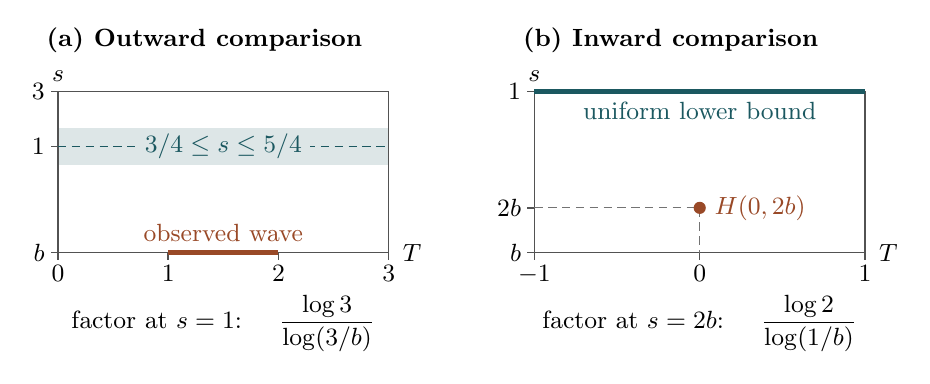
\begin{tikzpicture}[
  x=1cm,y=1cm,font=\small,inner sep=1.5pt,
  wall/.style={draw=black!68,line width=.55pt},
  guide/.style={draw=black!55,line width=.45pt,densely dashed},
  panel/.style={font=\small\bfseries,anchor=west,inner sep=0pt},
  ticklabel/.style={anchor=north,inner ysep=2pt}]
  % The radial coordinates are schematic; the horizontal coordinates give
  % the actual time windows for the two deterministic comparisons.
  \node[panel] at (-.15,2.7) {(a) Outward comparison};
  \fill[cylinderteal!15] (0,1.12) rectangle (4.2,1.58);
  \draw[wall] (0,0) rectangle (4.2,2.05);
  \draw[draw=cylinderteal,densely dashed,line width=.5pt]
    (0,1.35) -- (4.2,1.35);
  \node[fill=cylinderteal!15,inner xsep=3pt,text=cylinderteal]
    at (2.1,1.35) {$3/4\le s\le5/4$};
  \foreach \x/\t in {0/0,1.4/1,2.8/2,4.2/3}{
    \draw[wall] (\x,0) -- +(0,-.09);
    \node[ticklabel] at (\x,-.09) {$\t$};}
  \foreach \y/\s in {0/b,1.35/1,2.05/3}{
    \draw[wall] (0,\y) -- +(-.09,0);
    \node[anchor=east] at (-.11,\y) {$\s$};}
  \node[anchor=south] at (0,2.12) {$s$};
  \node[anchor=west] at (4.32,0) {$T$};
  \draw[draw=cylinderorange,line width=1.8pt] (1.4,0) -- (2.8,0);
  \node[text=cylinderorange,anchor=south] at (2.1,.08) {observed wave};
  \node at (2.1,-.90) {factor at $s=1$: \quad $\displaystyle\frac{\log 3}{\log(3/b)}$};
  \begin{scope}[xshift=6.05cm]
    \node[panel] at (-.15,2.7) {(b) Inward comparison};
    \draw[wall] (0,0) rectangle (4.2,2.05);
    \draw[guide] (0,.57) -- (2.1,.57) -- (2.1,0);
    \foreach \x/\t in {0/{-1},2.1/0,4.2/1}{
      \draw[wall] (\x,0) -- +(0,-.09);
      \node[ticklabel] at (\x,-.09) {$\t$};}
    \foreach \y/\s in {0/b,.57/{2b},2.05/1}{
      \draw[wall] (0,\y) -- +(-.09,0);
      \node[anchor=east] at (-.11,\y) {$\s$};}
    \node[anchor=south] at (0,2.12) {$s$};
    \node[anchor=west] at (4.32,0) {$T$};
    \draw[draw=cylinderteal,line width=1.8pt] (0,2.05) -- (4.2,2.05);
    \node[text=cylinderteal,anchor=north] at (2.1,1.97) {uniform lower bound};
    \fill[cylinderorange] (2.1,.57) circle[radius=2.2pt];
    \node[anchor=west,text=cylinderorange] at (2.23,.57) {$H(0,2b)$};
    \node at (2.1,-.90) {factor at $s=2b$: \quad $\displaystyle\frac{\log 2}{\log(1/b)}$};
  \end{scope}
\end{tikzpicture}
\caption{The two comparisons, with radii $s=|\tau|$ drawn schematically.
The boundary mass on $1\le T\le2$ bounds the mass in the shaded band
from below. The mean inequality on a fixed annulus supplies a lower bound
on the entire upper wall in~(b). The two displayed fractions are values
of the normalized radial harmonic functions. The comparison solutions
with potential dominate fixed multiples of these values, giving the
factor $[\log(3/b)]^{-2}$ at the dot. In the wave estimate, $b=2Kh$:
$H$ controls the wave norm on the marked segment and is controlled by
the initial data at the dot.}\label{fig:cylinder}
\end{figure}
